\documentclass[12pt]{article}
\usepackage{amsmath}
\usepackage{amsfonts}
\usepackage{amsthm}
\usepackage{amssymb}
\usepackage{algorithm}
\usepackage[english]{babel}
\usepackage{color}
\usepackage{float}
\usepackage[utf8]{inputenc}
\usepackage[margin=1 in]{geometry}
\usepackage{graphicx}
\usepackage{hyperref}
\usepackage{indentfirst}
\usepackage{titlesec}

% additional packages
\usepackage{subcaption}

\title{States Estimation of Li-ion Battery}
\author{Junzhe Shi, Franklin Zhao, Ruitong Zhu, and Xin Peng}
\date{}


\begin{document}

\maketitle

\maketitle
%%%%%%%%%%%%%%%%%%%%%%%%%%%%%%%%%%%%%%%%%%%%%%%%%%%%%%%%%%%%%%%%%%
\section*{Abstract}
%%%%%%%%%%%%%%%%%%%%%%%%%%%%%%%%%%%%%%%%%%%%%%%%%%%%%%%%%%%%%%%%%%

Batteries are ubiquitous in all forms of electronics and transportation, and a key to the store of clean and secure energy. For different kinds of batteries,  Li-ion battery is the most prominent one for their superior gravimetric and volumetric energy density.  For the safe operation of Li-ion battery, the state of charge (SOC) and state of health (SOH) estimation are of great significance. Hence, the goal of the project is to design a robust observer which can estimate the SOC and SOH of Li-ion batteries. In the project, the equivalent-circuit model is used for the battery modeling with current and ambient temperature as inputs and voltage as the measured output. The equivalent-circuit model includes three parts which are an electrical model, a thermal model, and an aging model. To ensure the accuracy of states estimation, the Extend Kalman Filter (EKF) is applied and examined in the project. The battery system is constructed and simulated using MATLAB. The best observer built in this project is a Voltage-Temperature (VT) observer which can accurately observe SOC with great robustness, while SOH can be observed using open-loop observer. The robustness of designed observer is tested using the wrong initial estimates and wrong model parameters.

%%%%%%%%%%%%%%%%%%%%%%%%%%%%%%%%%%%%%%%%%%%%%%%%%%%%%%%%%%%%%%%%%%
\section*{Introduction}
%%%%%%%%%%%%%%%%%%%%%%%%%%%%%%%%%%%%%%%%%%%%%%%%%%%%%%%%%%%%%%%%%%
\subsection*{Motivation and Background} 

The identification of battery operation and aging in real life has been a long-desired yet challenging goal, which includes multiple complex processes in complicated operating conditions and environments. An accurate method to observe SOC and SOH of Li-ion battery is in need. Meanwhile, batteries invariably work at varying thermal and aging conditions. Thus, it is necessary for us to build a battery observation system to monitor operation and aging of battery. The potential challenges also exist. We need to express a multi-control problem via mathematical equations and combine electrical model, thermal model and aging model. Besides, since all team members are major in Civil Systems, a lack of background knowledge in electrical engineering can be a big challenge. However, our previous course CE 291F, Control and Optimization of Distributed Parameters Systems can be helpful for the project. It gave us a background knowledge of partial differential equations, conservation laws, linear stability, Kalman filter and so on. We all have experiences of building, controlling and optimizing systems, including quench process,  heat diffusion and Lighthill Whitham Richards model.

\subsection*{Focus of this Study} 

In this project, we will focus on the SOC and SOH of Li-ion batteries. Based on equivalent-circuit, the electrical, thermal and aging models will be developed for the observing system. Since battery monitoring and management can be the key to allowing innovation in future designs because of their limit properties, our system may play an important role in such an area, and significantly contribute to the energy saving and efficiency.

\subsection*{Literature review} 

The behavior of batteries is difficult to predict because of its non-linearity, and there has been quite a few attempts to model and estimate the inner state of the system. To better describe the behavior of batteries, a lumped-parameter electro-thermal model was introduced to capture the correlation between the thermal and electric behavior \cite{ref:4}, a semi-empirical cycle-life model was established to investigate the attributes of capacity loss \cite{ref:3}. As a combination of the two models above, a coupled electro-thermal-aging model is developed in \cite{ref:1}, which captured the systematic dynamics for lithium-iron-phosphate batteries. This model provides a decent assumption for the battery behaviors, which we will go through in detail at the section of mathematical model, as well as an open-loop observer for the Sate of Charge (SOC) and State of Health (SOH). Inspired by the course material of CE 295, we tried to go further to investigate more possible approaches to estimate the battery states.


\subsection*{Key contributions} 

Based on the thermal-electrical-aging model as discussed above, we build a robust observer for the model, which provides users with an efficient method to monitor State of Charge and State of Health for battery.


%%%%%%%%%%%%%%%%%%%%%%%%%%%%%%%%%%%%%%%%%%%%%%%%%%%%%%%%%%%%%%%%%%
\section{Technical Description}
%%%%%%%%%%%%%%%%%%%%%%%%%%%%%%%%%%%%%%%%%%%%%%%%%%%%%%%%%%%%%%%%%%
\subsection{Mathematical Model}
Our analysis is based on a coupled electro-thermal-aging model for lithium-iron-phosphate batteries, which is introduced in \cite{ref:1}. 
The model consists of a two RC pair electrical model, a two-state thermal model and a semi-empirical aging model.
\subsubsection{Electrical Model}
As shown in Figure \ref{p1}, the electrical comprises an open-circuit voltage $(OCV, V_{OC})$, two resistor-capacitor (RC) pairs ($R_1$, $C_1$, $R_2$, $C_2$), and an ohmic resistor ($R_0$). The state-space model is given by:
\begin{equation}
\frac{\mathrm{d} SOC}{\mathrm{d}t}(t) = \frac{I(t)}{C_{bat}}
\end{equation}
\begin{equation}
\frac{\mathrm{d} V_1}{\mathrm{d}t}(t) = -\frac{V_1(t)}{R_1C_1}+\frac{I(t)}{C_1}
\end{equation}
\begin{equation}
\frac{\mathrm{d} V_2}{\mathrm{d}t}(t) = -\frac{V_2(t)}{R_2C_2}+\frac{I(t)}{C_2}
\end{equation}
\begin{equation}
V_t(t) = V_{OC}(SOC)+V_1(t)+V_2(t)+R_0I(t)
\end{equation}
where $C_{bat}$ is the nominal capacity of the battery, $I(t)$ is the current (positive for charging), and $V_t(t)$ denotes the terminal voltage. Three state variables are $SOC$ and voltages across the two RC pairs $V_1$, $V_2$. 
\begin{figure}[H]
	\centering
	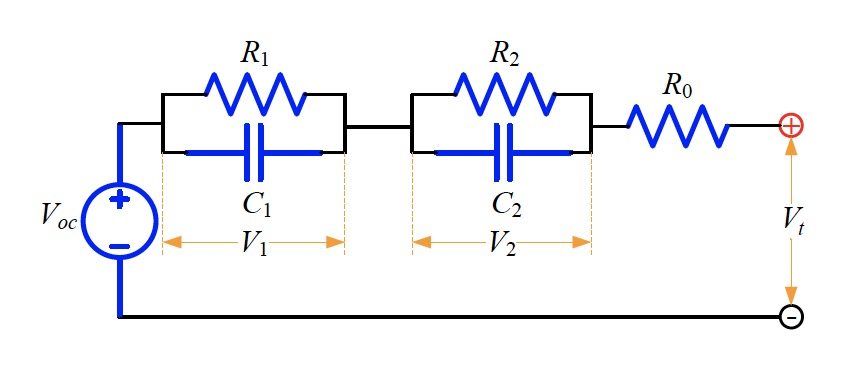
\includegraphics[height=0.3\textwidth]{figures/circuit.jpg}
	\caption{Electrical Model \cite{ref:1}}
	\label{p1}
\end{figure}
\noindent The electrical parameters are identified in \cite{ref:2}. In our model, we follow the equations listed in the appendix to derive these parameters based on the state of charge ($I<0$) or discharge ($I\ge 0$).

\subsubsection{Thermal Model}
\begin{figure}[H]
	\centering
	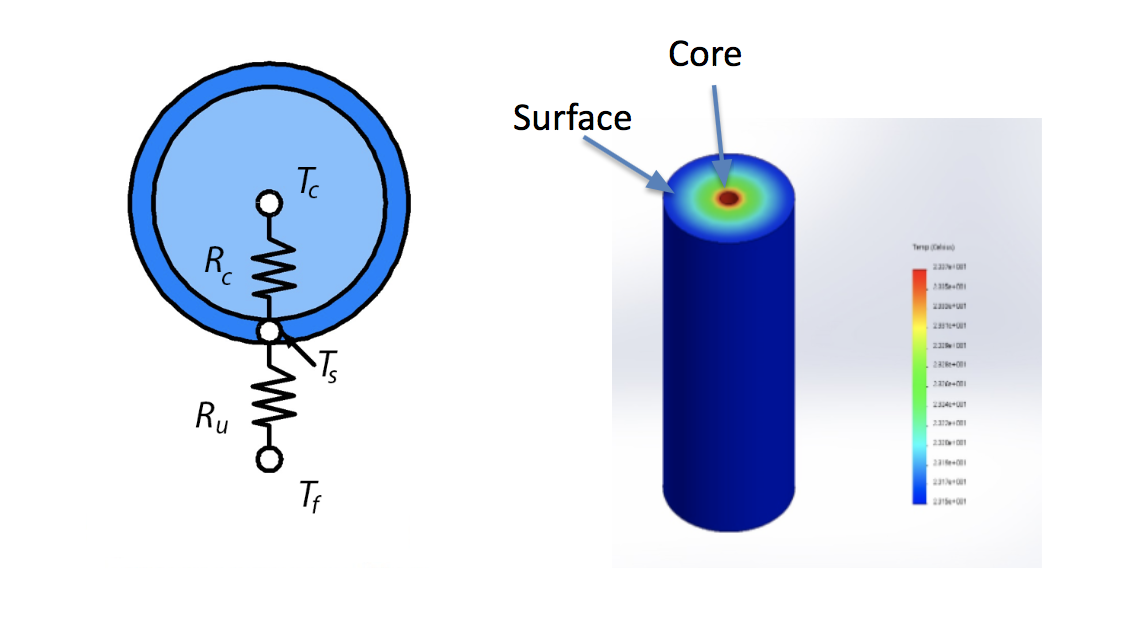
\includegraphics[height=0.3\textwidth]{figures/thermal.png}
	\caption{Two-state Thermal Model}
	\label{pi2}
\end{figure}
Since the core temperature can be higher than the surface temperature under high current rates \cite{ref:2}, a two-state thermal system was hereby introduced to capture both core and surface temperature dynamics. As sketched in Figure \ref{pi2}, the radial heat transfer dynamics of a cylindrical battery can be described as follow.
\begin{equation}
\frac{\mathrm{d}T_c(t)}{\mathrm{d} t} = \frac{T_s(t)-T_c(t)}{R_cC_c}+\frac{Q(t)}{C_c}
\end{equation}
\begin{equation}
\frac{\mathrm{d}T_s(t)}{\mathrm{d} t} = \frac{T_f(t)-T_s(t)}{R_uC_s}+\frac{T_s(t)-T_c(t)}{R_cC_s}
\end{equation}
$R_c$, $R_u$, $C_c$ and $C_s$ represent the heat conduction resistance, convection resistance, core heat capacity and surface heat capacity respectively, with their values shown in Table \ref{t5}; two state variables are core temperature $T_c$ and surface temperature $T_s$; the ambient temperature $T_f$ is treated as uncontrollable input. 
\begin{table}[H]
	\caption{Thermal Parameters}
	\vspace{-0.4cm}
	\centering
	\begin{tabular}{llll}
		\hline
		$R_{c}(KW^{-1})$ & $R_{u}(KW^{-1})$ & $C_{c}(JK^{-1})$ & $C_{s}(JK^{-1})$ \\
		\hline
		1.94 & 3.08 & 62.7 & 4.5  \\
		\hline
	\end{tabular}
	\label{t5}
\end{table}
\noindent $Q(t)=|I(V_{OC}-V_t)|$ is heat generation including joule heating and energy dissipated by electrode over-potentials, based on equation (4), we can rewrite equation (5) as
\begin{equation}
\frac{\mathrm{d}T_c(t)}{\mathrm{d} t} = \frac{T_s(t)-T_c(t)}{R_cC_c}+\frac{I(t)(V_1(t)+V_2(t)+R_0I(t)}{C_c}
\end{equation}
\subsubsection{Aging Model}
The aging model is based upon a matrix of cycling tests from \cite{ref:3}. The experiment results suggest that capacity fade depends strongly on C-rate and temperature in the cell at low charge/discharge rates, while the sensitivity to depth-of-discharge is negligible. The semi-empirical life model adopted the following equation to describe the correlation between the capacity loss ($\Delta Q_b$, in $\%$) and the discharged Ah throughput($A$, depends on C-rate),
\begin{equation}
\Delta Q_b = M(c)\mathrm{exp}\left(\frac{-E_a(c)}{RT_c}\right)A(c)^z
\end{equation}
where $M(c)$ is the pre-exponential factor as a funciton of C-rate, which is denoted by $c$. The relation between the pre-exponential factor $M(c)$ and C-rate are shown in Table \ref{t6}. The activation energy $E_a$ and the power-law factor $z$ are given by
\begin{equation}
E_a(c)=31700-370.3c  \quad z=0.55
\end{equation}
\begin{table}[H]
	\caption{Pre-exponential Factor as a function of the C-rate}
	\vspace{-0.4cm}
	\centering
	\begin{tabular}{lllll}
		\hline
		C-rate c & 0.5 & 2 & 6 & 10 \\
		\hline
		M & 31630 & 21681 & 12934 & 15512  \\
		\hline
	\end{tabular}
	\label{t6}
\end{table}
\noindent The model consider a capacity loss of $20\%$ as the end-of-life (EOL) for an automotive battery. The corresponding Ah throughput $A_{tol}$ and the number of cycles $N$ are therefore calculated as below.
\begin{equation}
A_{tol} (c, T_c) = \left[ \frac{20}{M(c)\mathrm{exp}\left(\frac{-E_a(c)}{RT_c}\right)} \right]^{\frac{1}{z}}
\end{equation}
\begin{equation}
N(c, T_c) = \frac{3600A_{tol} (c, T_c) }{C_{bat}}
\end{equation}
Each cycle correspondes to $2C_{bat}$ charge throughput, and since $A_{tol}$ is discharged Ah throughput, the total throughput including both charged and discharged Ah should be $2A_{tol}$. Based on this, the battery State-of-Health (SOH) is defined as: 
\begin{equation}
SOH(t) = SOH(t_0)-\frac{\int_{t_0}^{t}|I(\tau)\mathrm{d}\tau}{2N(c, T_c) C_{bat}}
\end{equation}
where $t_0$ denotes the initial time. $SOH$ varies among $[0,1]$, $SOH=1$ correspondes to a brand new battery and $SOH=0$  means $20\%$ capacity loss, as known as EOL. The derivative of $SOH$ yields the battery aging model
\begin{equation}
\frac{\mathrm{d} SOH}{\mathrm{d}t}(t) = -\frac{|I(t)|}{2N(c, T_c) C_{bat}}
\end{equation}
\subsubsection{Model Coupling}
\begin{figure}[H]
	\centering
	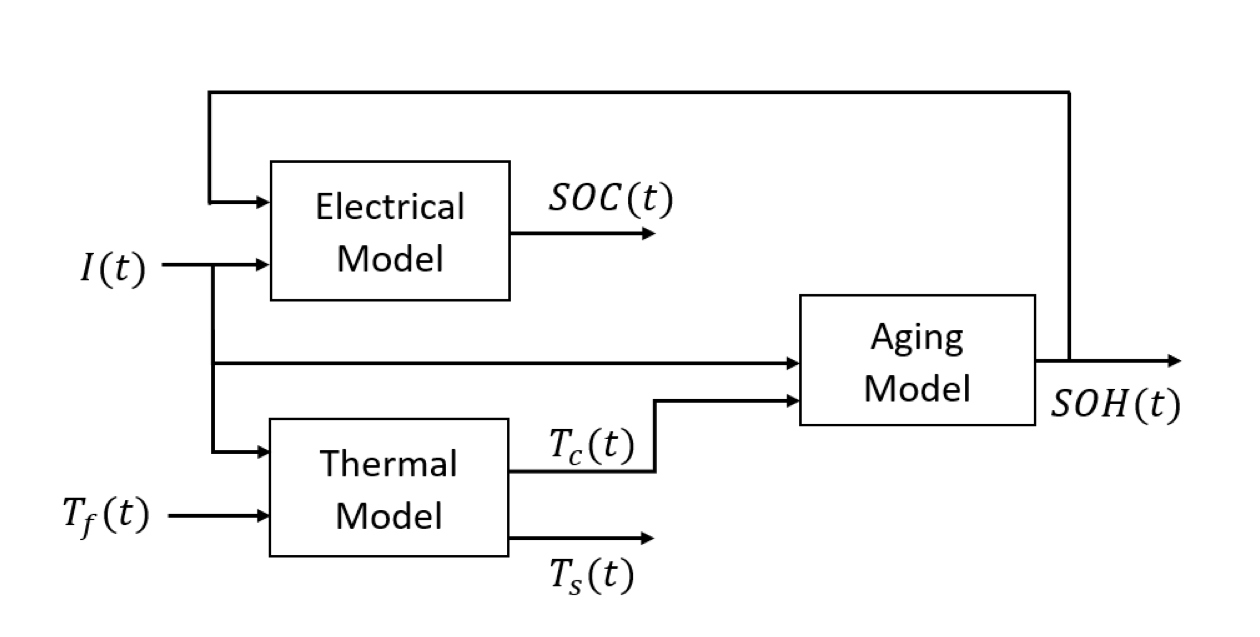
\includegraphics[height=0.3\textwidth]{figures/coupling.png}
	\caption{Electro-Thermal-Aging Model Coupling}
	\label{p2}
\end{figure}
\noindent Combining the above three subsystems, the model dynamics are summarized as below.
\begin{equation}
\frac{\mathrm{d} SOC}{\mathrm{d}t}(t) = \frac{I(t)}{C_{bat}}
\end{equation}
\begin{equation}
\frac{\mathrm{d} V_1}{\mathrm{d}t}(t) = -\frac{V_1(t)}{R_1C_1}+\frac{I(t)}{C_1}
\end{equation}
\begin{equation}
\frac{\mathrm{d} V_2}{\mathrm{d}t}(t) = -\frac{V_2(t)}{R_2C_2}+\frac{I(t)}{C_2}
\end{equation}
\begin{equation}
\frac{\mathrm{d}T_c(t)}{\mathrm{d} t} = \frac{T_s(t)-T_c(t)}{R_cC_c}+\frac{I(t)(V_1(t)+V_2(t)+R_0I(t)}{C_c}
\end{equation}
\begin{equation}
\frac{\mathrm{d}T_s(t)}{\mathrm{d} t} = \frac{T_f(t)-T_s(t)}{R_uC_s}+\frac{T_s(t)-T_c(t)}{R_cC_s}
\end{equation}
\begin{equation}
\frac{\mathrm{d} SOH}{\mathrm{d}t}(t) = -\frac{|I(t)|}{2N(c, T_c) C_{bat}}
\end{equation}
\noindent Inputs in this model include current $I_(t)$, which is controllable, and ambient temperature $T_f(t)$, which is uncontrollable. 


\subsection{Observer \& Simulation}
All the parameters used in this project base on the parameter of an A123 Li-ion battery. In the 1 hour of simulation, the controllable input is charging rate which is a constant value $0.9 C$. The uncontrollable input, ambient temperature, is assumed as a half sine wave. The input values are presented in Figure~\ref{fig:sysInput}.
\begin{figure}[H]
	\centering
	\begin{subfigure}[t]{0.45\linewidth}
		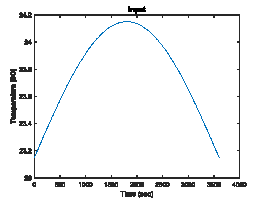
\includegraphics[width=\linewidth]{figures/sysinput1.pdf}
	\end{subfigure}
	\begin{subfigure}[t]{0.45\linewidth}
		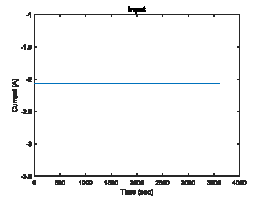
\includegraphics[width=\linewidth]{figures/sysinput2.pdf}
	\end{subfigure}	
	\caption{Systems inputs}\label{fig:sysInput}
\end{figure}
In the simulation outputs, SOC reached 90\% after 1-hour charging. The terminal voltage also increases as the SOC increases. SOH decreased as the time goes by. The core and surface temperatures of Li-ion battery changed under the effects of the current and the ambient temperature. The simulation outputs are showed in Figure~\ref{fig:sysOutput}.
\begin{figure}[H]
	\centering
	\begin{subfigure}[t]{0.45\linewidth}
		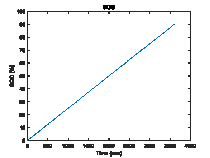
\includegraphics[width=\linewidth]{figures/sysOutput1.pdf}
	\end{subfigure}
	\begin{subfigure}[t]{0.45\linewidth}
		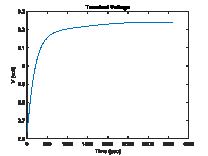
\includegraphics[width=\linewidth]{figures/sysOutput2.pdf}
	\end{subfigure}	
	\begin{subfigure}[t]{0.45\linewidth}
		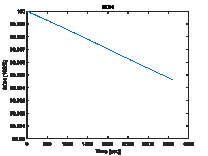
\includegraphics[width=\linewidth]{figures/sysOutput3.pdf}
	\end{subfigure}
	\begin{subfigure}[t]{0.45\linewidth}
		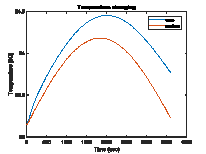
\includegraphics[width=\linewidth]{figures/sysOutput4.pdf}
	\end{subfigure}	
	\caption{Systems outputs}\label{fig:sysOutput}
\end{figure}
By adding white noises in the terminal voltage and surface temperature data with SNR is equal to 60, the synthetic data is generated from this simulation model to produce measurements of terminal voltage and surface temperature. The synthetic measurements are presented in Figure~\ref{fig:measureOut}.
\begin{figure}[H]
	\centering
	\begin{subfigure}[t]{0.45\linewidth}
		\includegraphics[width=\linewidth]{figures/measureOut1.pdf}
	\end{subfigure}
	\begin{subfigure}[t]{0.45\linewidth}
		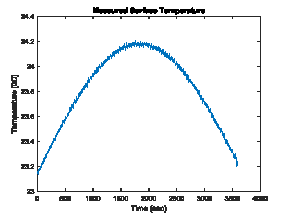
\includegraphics[width=\linewidth]{figures/measureOut2.pdf}
	\end{subfigure}	
	\caption{Measured outputs}\label{fig:measureOut}
\end{figure}
By using Extended Kalman Filter method, three different observers are created. The components of these three observers are showed on Table~\ref{tb:3obs}.
\begin{table}[H]
	\caption{Three observers}
	\vspace{-0.4cm}
	\label{tb:3obs}
	\centering
	\begin{tabular}{ccc}
		\hline
		\textbf{Observers}&\textbf{Control inputs}&\textbf{Measured inputs}\\
		\hline
		Voltage-measured observer&$T_f$, Current&$V_T$ \\
		Temperature-measured observer&$T_f$, Current&$T_S$\\
		VT-measured observer&$T_f$, Current&$V_T$, $T_S$\\
		\hline
	\end{tabular}
\end{table}
In order to test the robustness of the three observers, these observers were tested with wrong initial estimates and wrong parameter values respectively. 
\subsubsection{Voltage-measured observer}
The test results of the Voltage-measured observer with wrong initial estimates and wrong parameter values in showed in Figure~\ref{fig:estVoltIni} and Figure~\ref{fig:estVoltPar} respectively.
\begin{figure}[H]
	\centering
	\begin{subfigure}[t]{0.3\linewidth}
		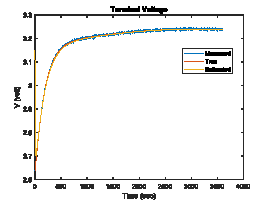
\includegraphics[width=\linewidth]{figures/estVoltIni1.pdf}
	\end{subfigure}
	\begin{subfigure}[t]{0.3\linewidth}
		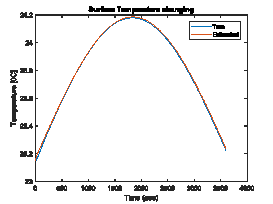
\includegraphics[width=\linewidth]{figures/estVoltIni2.pdf}
	\end{subfigure}	
	\begin{subfigure}[t]{0.3\linewidth}
		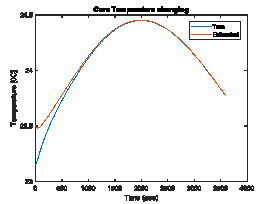
\includegraphics[width=\linewidth]{figures/estVoltIni3.pdf}
	\end{subfigure}
	\begin{subfigure}[t]{0.3\linewidth}
		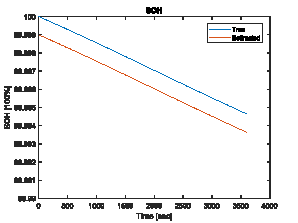
\includegraphics[width=\linewidth]{figures/estVoltIni4.pdf}
	\end{subfigure}	
	\begin{subfigure}[t]{0.3\linewidth}
		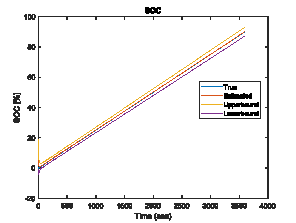
\includegraphics[width=\linewidth]{figures/estVoltIni5.pdf}
	\end{subfigure}	
	\caption{Estimation test of voltage-measured observer with wrong initial values}\label{fig:estVoltIni}
\end{figure}
\begin{figure}[H]
	\centering
	\begin{subfigure}[t]{0.3\linewidth}
		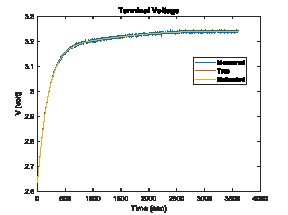
\includegraphics[width=\linewidth]{figures/estVoltPar1.pdf}
	\end{subfigure}
	\begin{subfigure}[t]{0.3\linewidth}
		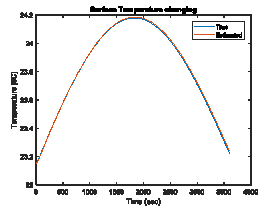
\includegraphics[width=\linewidth]{figures/estVoltPar2.pdf}
	\end{subfigure}	
	\begin{subfigure}[t]{0.3\linewidth}
		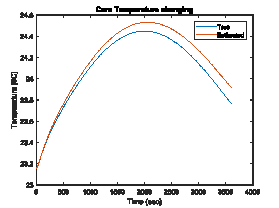
\includegraphics[width=\linewidth]{figures/estVoltPar3.pdf}
	\end{subfigure}
	\begin{subfigure}[t]{0.3\linewidth}
		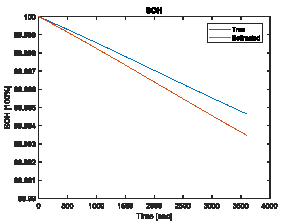
\includegraphics[width=\linewidth]{figures/estVoltPar4.pdf}
	\end{subfigure}	
	\begin{subfigure}[t]{0.3\linewidth}
		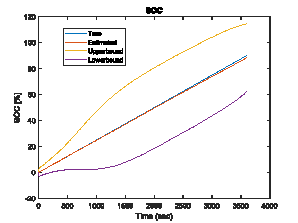
\includegraphics[width=\linewidth]{figures/estVoltPar5.pdf}
	\end{subfigure}	
	\caption{Estimation test of voltage-measured observer with wrong parameters }\label{fig:estVoltPar}
\end{figure}
For the voltage-measured observer, the SOC and terminal voltage are well estimated. The estimated surface and core temperatures of battery converge with their true values after 1000 seconds. The estimated SOH does not converge to it true value at all. The result shows that SOH is unobservable. It is because the observability matrix of the voltage-measured observer is not full rank. The null space to the observability matrix is span($[0,0,0,1,0,0]^T$, $[0,0,0,0,1,0]^T$, $[0,0,0,0,1]^T$). It means the states of $T_c$, $T_s$, and SOH are unobservable for this observer. However, when the observer's model is very accurate, the temperatures will converge to their true values, even if temperatures are unobservable for the voltage-measured observer. It is because the thermal system is asymptotically stable, the surface and core temperatures will reach their equilibrium states after a long time. 
\subsubsection{Temperature-measured observer}
The test results of the Temperature-measured observer with wrong initial estimates and wrong parameter values in showed in Figure~\ref{fig:estTempIni} and Figure~\ref{fig:estTempPar} respectively.
\begin{figure}[H]
	\centering
	\begin{subfigure}[t]{0.3\linewidth}
		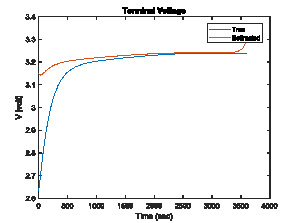
\includegraphics[width=\linewidth]{figures/estTempIni1.pdf}
	\end{subfigure}
	\begin{subfigure}[t]{0.3\linewidth}
		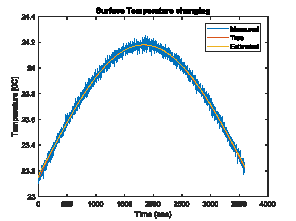
\includegraphics[width=\linewidth]{figures/estTempIni2.pdf}
	\end{subfigure}	
	\begin{subfigure}[t]{0.3\linewidth}
		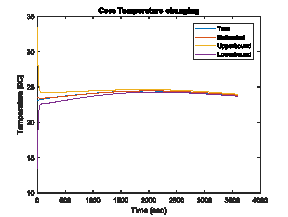
\includegraphics[width=\linewidth]{figures/estTempIni3.pdf}
	\end{subfigure}
	\begin{subfigure}[t]{0.3\linewidth}
		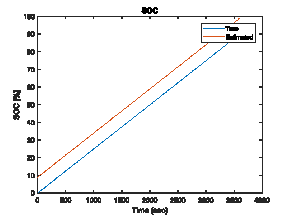
\includegraphics[width=\linewidth]{figures/estTempIni4.pdf}
	\end{subfigure}	
	\begin{subfigure}[t]{0.3\linewidth}
		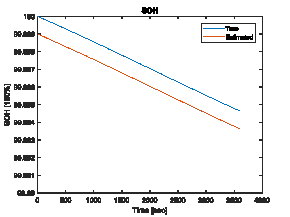
\includegraphics[width=\linewidth]{figures/estTempIni5.pdf}
	\end{subfigure}	
	\caption{Estimation test of temperature-measured observer with wrong initial values}\label{fig:estTempIni}
\end{figure}
\begin{figure}[H]
	\centering
	\begin{subfigure}[t]{0.3\linewidth}
		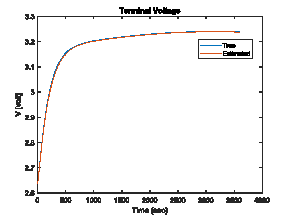
\includegraphics[width=\linewidth]{figures/estTempPar1.pdf}
	\end{subfigure}
	\begin{subfigure}[t]{0.3\linewidth}
		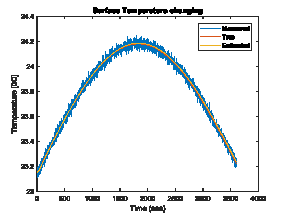
\includegraphics[width=\linewidth]{figures/estTempPar2.pdf}
	\end{subfigure}	
	\begin{subfigure}[t]{0.3\linewidth}
		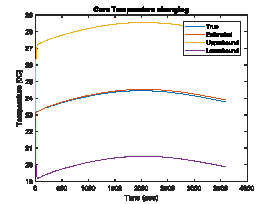
\includegraphics[width=\linewidth]{figures/estTempPar3.pdf}
	\end{subfigure}
	\begin{subfigure}[t]{0.3\linewidth}
		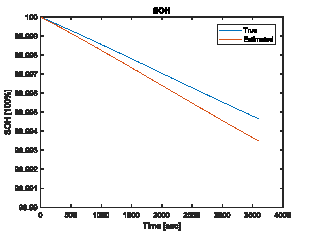
\includegraphics[width=\linewidth]{figures/estTempPar4.pdf}
	\end{subfigure}	
	\begin{subfigure}[t]{0.3\linewidth}
		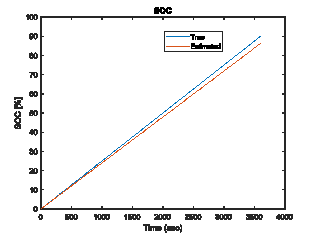
\includegraphics[width=\linewidth]{figures/estTempPar5.pdf}
	\end{subfigure}	
	\caption{Estimation test of temperature-measured observer with wrong parameters }\label{fig:estTempPar}
\end{figure}
For the temperature-measured observer, the surface and core temperatures of the battery are well estimated. The estimated SOC and SOH does not converge to their true values. The test result shows that SOC and SOH are unobservable for the temperature-measured observer. The rank of the observability matrix of the observer is 4 which is not full rank. The null space to the observability matrix is span($[1,0,0,0,0,0]^T$, $[0,0,0,0,0,1]^T$). The null space also indicates the unobservability of SOC and SOH for temperature-measured observer. 
\subsubsection{Voltage and temperature (VT) -measured observer}
The test results of the VT-measured observer with wrong initial estimates and wrong parameter values in showed in Figure~\ref{fig:estVTini} and Figure~\ref{fig:estVTpar} respectively.
\begin{figure}[H]
	\centering
	\begin{subfigure}[t]{0.3\linewidth}
		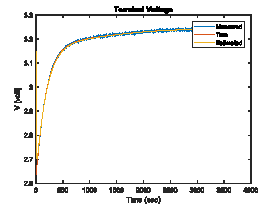
\includegraphics[width=\linewidth]{figures/estVTini1.pdf}
	\end{subfigure}
	\begin{subfigure}[t]{0.3\linewidth}
		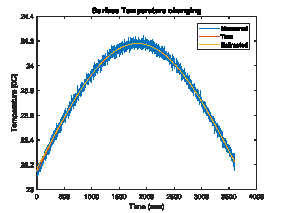
\includegraphics[width=\linewidth]{figures/estVTini2.pdf}
	\end{subfigure}	
	\begin{subfigure}[t]{0.3\linewidth}
		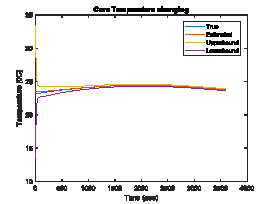
\includegraphics[width=\linewidth]{figures/estVTini3.pdf}
	\end{subfigure}
	\begin{subfigure}[t]{0.3\linewidth}
		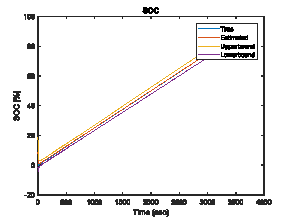
\includegraphics[width=\linewidth]{figures/estVTini4.pdf}
	\end{subfigure}	
	\begin{subfigure}[t]{0.3\linewidth}
		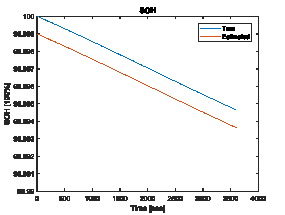
\includegraphics[width=\linewidth]{figures/estVTini5.pdf}
	\end{subfigure}	
	\caption{Estimation test of VT-measured observer with wrong initial values }\label{fig:estVTini}
\end{figure}
\begin{figure}[H]
	\centering
	\begin{subfigure}[t]{0.3\linewidth}
		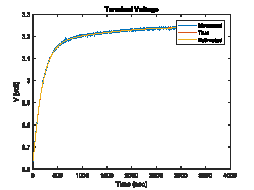
\includegraphics[width=\linewidth]{figures/estVTpar1.pdf}
	\end{subfigure}
	\begin{subfigure}[t]{0.3\linewidth}
		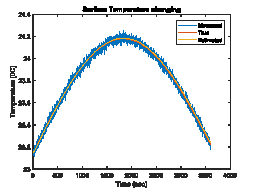
\includegraphics[width=\linewidth]{figures/estVTpar2.pdf}
	\end{subfigure}	
	\begin{subfigure}[t]{0.3\linewidth}
		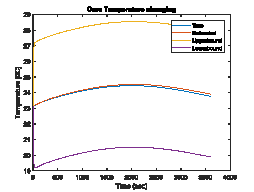
\includegraphics[width=\linewidth]{figures/estVTpar3.pdf}
	\end{subfigure}
	\begin{subfigure}[t]{0.3\linewidth}
		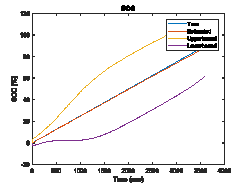
\includegraphics[width=\linewidth]{figures/estVTpar4.pdf}
	\end{subfigure}	
	\begin{subfigure}[t]{0.3\linewidth}
		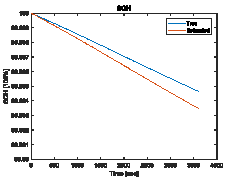
\includegraphics[width=\linewidth]{figures/estVTpar5.pdf}
	\end{subfigure}	
	\caption{Estimation test of VT-measured observer with wrong parameters 
	}\label{fig:estVTpar}
\end{figure}
For the VT-measured observer, $V_T$, $T_C$, $T_S$, and SOC of the battery are well estimated, except the SOH. The rank of the observability matrix of the observer is 5. The null space to the observability matrix is the span($[0,0,0,0,0,1]^T$) which also indicates the unobservability of the SOH.
\subsubsection{Comparsion}
To better evaluate the performance of these three kinds of observers, the observability of 6 battery states of the observers are presented on Table~\ref{tb:ob?}. The root-mean-squared error (RMSE) of three observers and two tests are showed on Table~\ref{tb:rmseIni} and Table~\ref{tb:rmsePar}.
\begin{table}[H]
	\caption{The observability three observers}
	\vspace{-0.4cm}
	\label{tb:ob?}
	\centering
	\begin{tabular}{ccccccc}
		\hline
		\textbf{Observers}&\textbf{SOC\%}&$\bf{V_1}$&$\bf{V_2}$&$\bf{T_S}$&$\bf{T_C}$&\textbf{SOH\%}\\
		\hline
		Voltage-measured observer&Yes&Yes&Yes&No&No&No\\
		Temperature-measured observer&No&Yes&Yes&Yes&Yes&No\\
		VT-measured observer&Yes&Yes&Yes&Yes&Yes&No\\
		\hline
	\end{tabular}
\end{table}
\begin{table}[H]
	\caption{RMSE of Extended Kalman Filter with wrong initial values}
	\vspace{-0.4cm}
	\label{tb:rmseIni}
	\centering
	\begin{tabular}{cccccc}
		\hline
		\textbf{Observers}&$\bf{V_T}$&$\bf{T_S}$&$\bf{T_C}$&\textbf{SOC\%}&\textbf{SOH\%}\\
		\hline
		Voltage-measured observer&0.0163&0.0060&0.0607&0.2848&0.1009\\
		Temperature-measured observer&0.0861&0.0055&0.0554&51.3642&0.1004\\
		VT-measured observer&0.1063&0.0059&0.0594&0.2758&0.1009\\
		\hline
	\end{tabular}
\end{table}
\begin{table}[H]
	\caption{RMSE of Extended Kalman Filter with wrong parameters in models}
	\vspace{-0.4cm}
	\label{tb:rmsePar}
	\centering
	\begin{tabular}{cccccc}
		\hline
		\textbf{Observers}&$\bf{V_T}$&$\bf{T_S}$&$\bf{T_C}$&\textbf{SOC\%}&\textbf{SOH\%}\\
		\hline
		Voltage-measured observer&0.0004&0.0090&0.0878&0.7590&0.0669\\
		Temperature-measured observer&0.0034&0.0078&0.0798&51.4638&0.0669\\
		VT-measured observer&0.0004&0.0083&0.0848&0.7551&0.0669\\
		\hline
	\end{tabular}
\end{table}
\section{Discussion}
As the results shown in the previous part, for temperature observer, SOC, SOH is unobservable. For voltage observer, $T_C$, $T_S$, $SOH$ are unobservable. However, the temperature can be affected by the resistance of the circuit. On the other hand, the resistance will be affected by the temperature as well. Hence, the voltage observer can actually ``observe" $T_c$ and $T_S$ by an indirect approach since after a long time, the temperature would converge. 

Hence, we dicided to combine the templeature observer and voltage observer together as a VT-observer. As the results are shown, VT-measured observer has an overwhelming advantage. The observer can estimate most of the states because it the combines both V-measured observer and T-measured observer. In this project, there is not any observer can estimate the SOH. However, if an accurate battery model and initial values can be provided, the SOH values can be well estimated by an open-loop observer.

In addition, from the simulation result we notice that SOC has a positive linear relationship with charging time while SOH has a negative linear relationship with charging time. In the simulation, it requires nearly 2 hours to replenish the SOC from 0\% to 90\%, with the associated 0.005\% SOH decay. The highest SOC is 87.4\%, and the lowest SOH is 99.995\% compared to the original status. Such a trend indicates that charging time and battery health is a trade off. This is interesting, since a balance between efficiency and safety, is raised. If the highest efficency is needed, then the charging time should be minimized; If the highest safety is needed, then the aging condition should be minimized. However, in real-word cases, a balance point need should be find in different scenarios, which leads to a new topic -- optimal control for battery charging. Since batteries are storing most of the energy that we use in our daliy life, the observer we developed, as such a useful tool for the optimal control problems, will definitiely advance sustainablity in energy systems. Hence it can be noticed that state estimation is a really powerful tool for maintaining the energy system. In the future, a student team can focus on optimal control of the battery charging, based on the observer we developed.

%%%%%%%%%%%%%%%%%%%%%%%%%%%%%%%%%%%%%%%%%%%%%%%%%%%%%%%%%%%%%%%%%%
\section*{Executive Summary}
%%%%%%%%%%%%%%%%%%%%%%%%%%%%%%%%%%%%%%%%%%%%%%%%%%%%%%%%%%%%%%%%%%
In this project, we built the electric model, thermal model, and aging model, and implemented the open-loop simulation as well as state estimation using EKF. The goal of this project is to develop a battery observing system with high efficiency and robustness. Since with the accurate initial values and model parameters, the open-loop observer can observe the SOC and SOH pretty well, the trend of those curves are exactly as we expected. However, with wrong inital estimates and wrong parameter values, SOC cannot be observed by temperature observer, and SOH cannot be observed by both observers. Hence, for SOC in this scenario, it can be well-observed using our VT-observer; SOH can be observed using open-loop observer with correct initial estimates and parameters. Future work will focus on the optimal control of battery charging based on these observers we developed. 

\bibliographystyle{IEEEtran}%Used BibTeX style is unsrt
\bibliography{reference}

%%%%%%%%%%%%%%%%%%%%%%%%%%%%%%%%%%%%%%%%%%%%%%%%%%%%%%%%%%%%%%%%%%
\section*{Appendix}
%Should not be more than 2 or 3 pages.
%%%%%%%%%%%%%%%%%%%%%%%%%%%%%%%%%%%%%%%%%%%%%%%%%%%%%%%%%%%%%%%%%%
The parameters of equation (1)-(4) are identified as follow \cite{ref:2}, which varied across the state of charge ($I<0$) or discharge ($I\ge 0$).
\begin{equation}
R_{1} = \begin{Bmatrix}
R_{1d}&I\ge 0\\
R_{1c} &I<0
\end{Bmatrix}    
\end{equation}
\begin{equation}
R_{1_{*}}=(R_{10_{*}}+R_{11_{*}}(SOC)+R_{12_{*}}(SOC)^{2})exp\left ( \frac{T_{refR_{1}*}}{T_m-T_{shiftR_{1}*}} \right )
\end{equation}
\begin{table}[H]
	\caption{PARAMETRIC \ $R_1$ \ FUNCTION PARAMETERS}
	\vspace{-0.4cm}
	\centering
	\begin{tabular}{lllll}
		\hline
		$R_{10_{d}}$ & $R_{10_{c}}$ & $R_{11_{d}}$ & $R_{11_{c}}$ &$R_{12_{d}}$  \\
		\hline
		7.1135e-4 & 0.0016 & -4.3865e-4 & -0.0032 & 2.3788e-4 \\
		\hline
		$R_{12_{c}}$ & $T_{refR_{1}d}$& $T_{refR_{1}c}$ &$T_{shiftR_{1}d}$ & $T_{shiftR_{1}c}$\\
		\hline
		0.0045 & 347.4707 & 159.2819 & -79.5816 & -41.4578 \\
		\hline
	\end{tabular}
\end{table}
\begin{equation}
R_{2} = 
\begin{Bmatrix}
R_{2d}&I\ge 0\\
R_{2c} &I<0
\end{Bmatrix}
\end{equation}
\begin{equation}
R_{2_{*}}=(R_{20_{*}}+R_{21_{*}}(SOC)+R_{22_{*}}(SOC)^{2})exp\left ( \frac{T_{refR_{2}*}}{T_m} \right )
\end{equation}
\begin{table}[H]
	\caption{PARAMETRIC \ $R_2$ \ FUNCTION PARAMETERS}
	\vspace{-0.4cm}
	\centering
	\begin{tabular}{llll}
		\hline
		$R_{20_{d}}$ & $R_{20_{c}}$ & $R_{21_{d}}$ & $R_{21_{c}}$ \\
		\hline
		0.0288 & 0.0113 & -0.073 & -0.027  \\
		\hline
		$R_{22_{d}}$ & $R_{22_{c}}$& $T_{refR_{2}d}$& $T_{refR_{2}c}$ \\
		\hline
		0.0605 & 0.0339 & 16.6712 & 17.0224 \\
		\hline
	\end{tabular}
\end{table}
\begin{equation}
C_{1} = 
\begin{Bmatrix}
C_{1d}&I\ge 0 \\
C_{1c} &I<0
\end{Bmatrix}
\end{equation}
\begin{equation}
C_{1_{*}}=C_{10_{*}}+C_{11_{*}}(SOC)+C_{12_{*}}(SOC)^{2}+(C_{13_{*}}+C_{14_{*}}(SOC)+C_{15_{*}}(SOC)^{2}){T_m}
\end{equation}
\begin{table}[H]
	\caption{PARAMETRIC \ $C_1$ \  FUNCTION PARAMETERS}
	\vspace{-0.4cm}
	\centering
	\begin{tabular}{llll}
		\hline
		$C_{10_{d}}$ & $C_{10_{c}}$ & $C_{11_{d}}$ & $C_{11_{c}}$ \\
		\hline
		335.4518 & 523.215 & 3.1712e+3 & 6.4171e+3  \\
		\hline
		$C_{12_{d}}$ & $C_{12_{c}}$ & $C_{13_{d}}$ & $C_{13_{c}}$ \\
		\hline
		-1.3214e+3 & -7.5555e+3 & 53.2138 & 50.7107 \\
		\hline
		$C_{14_{d}}$ & $C_{14_{c}}$ & $C_{15_{d}}$ & $C_{15_{c}}$ \\
		\hline
		-65.4786 & -131.2298 & 44.3761 & 162.4688 \\
		\hline
	\end{tabular}
\end{table}
\begin{equation}
C_{2} = 
\begin{Bmatrix}
C_{2d}&I\ge 0  \\
C_{2c} &I<0
\end{Bmatrix}
\end{equation}
\begin{equation}
C_{2_{*}}=C_{20_{*}}+C_{21_{*}}(SOC)+C_{22_{*}}(SOC)^{2}+(C_{23_{*}}+C_{24_{*}}(SOC)+C_{25_{*}}(SOC)^{2}){T_m}
\end{equation}
\begin{table}[H]
	\caption{PARAMETRIC \ $C_1$ \ FUNCTION PARAMETERS}
	\vspace{-0.4cm}
	\centering
	\begin{tabular}{llll}
		\hline
		$C_{20_{d}}$ & $C_{20_{c}}$ & $C_{21_{d}}$ & $C_{21_{c}}$ \\
		\hline
		3.1887e+4 & 6.2449e+4 & -1.1593e+5 & -1.055e+5  \\
		\hline
		$C_{22_{d}}$ & $C_{22_{c}}$ & $C_{23_{d}}$ & $C_{23_{c}}$ \\
		\hline
		1.0493e+5 & 4.4432e+4 & 60.3114 & 198.9753 \\
		\hline
		$C_{24_{d}}$ & $C_{24_{c}}$ & $C_{25_{d}}$ & $C_{25_{c}}$ \\
		\hline
		1.0175e+4 & 7.5921e+3 & -9.5924e+3 & -6.9365e+3 \\
		\hline
	\end{tabular}
\end{table}

%%%%%%%%%%%%%%%%%%%%%%%%%%%%%%%%%%%%%%%%%%%%%%%%%%%%%%%%%%%%%%%%%%

\section*{Acknowledgments}
%%%%%%%%%%%%%%%%%%%%%%%%%%%%%%%%%%%%%%%%%%%%%%%%%%%%%%%%%%%%%%%%%%
\textit{The authors would like to thank Professor Scott Moura for guidance in this project.}


%%%%%%%%%%%%%%%%%%%%%%%%%%%%%%%%%%%%%%%%%%%%%%%%%%%%%%%%%%%%%%%%%%
\section*{About the authors}
%%%%%%%%%%%%%%%%%%%%%%%%%%%%%%%%%%%%%%%%%%%%%%%%%%%%%%%%%%%%%%%%%%
\begin{description}
    \item[Junzhe Shi] is a Systems Engineering student (Master of Science) at University of California, Berkeley.
    \item[Franklin Zhao] is a Systems Engineering student (Master of Science) at University of California, Berkeley. 
    \item[Ruitong Zhu] is a Systems Engineering student (Master of Science) at University of California, Berkeley. 
    \item[Xin Peng] is a Systems Engineering student (Master of Engineering) at University of California, Berkeley. 
\end{description}

\end{document}

